\section{Implémentation du modèle par champs léxical}

- En premier lieu nous nous sommes penchés sur la fréquence des mots pour savoir quelles sont les mots les plus fréquents dans un résumé de film par rapport à son genre.

Par exemple le genre \textbf{Horror}: \\
\begin{center}
    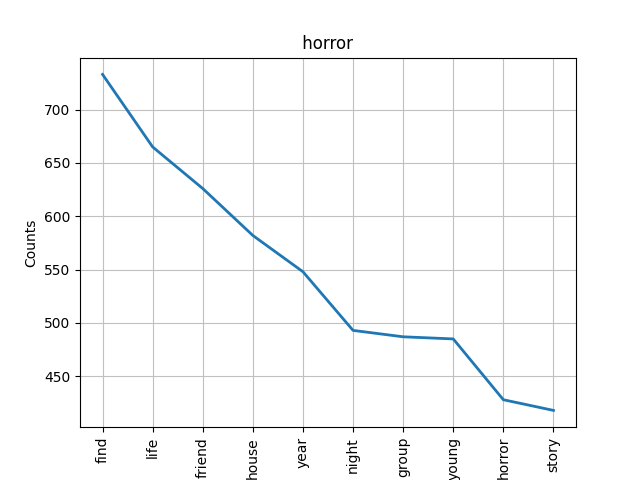
\includegraphics[scale=.8]{graphs/horror .png}
    \captionof{figure}{Horror genre words frequency}
\end{center}




- Nous avons ensuite créé une base de données du champ lexical de chaque genre.
Maintenant l'idée était de compter le nombre de mots qui appartenait au champ lexical de tous les genres que nous avions dans la base de données.\\
- De ça nous prenions le genre qui avait le plus de mot appartenant à son champ lexical.
Malheureusement cette classification a été un échec total et nous avions un taux d'erreur de 100\%. \\
Notre supposition serait que la base de données pourrait surement être la cause d’autant d’erreurs car beaucoup de mots doivent être manquant et un même mot ce retrouve dans plusieurs genre ce qui fausse les résultats.\\
